In this project, we are proposing a design of a PD controller to stabilize a ball on a tilting grooved system. 
The goal is to keep the ball in the vicinity of the origin that is around the shaft of the motor that controls the system. A sample illustration of this system can be seen from Figure \ref{fig:illustration}. In order to accomplish this task, firstly, the transfer function of the plant is derived using Newton's law and transferred into frequency domain by Laplace transform. \\

\begin{figure}[H]
    \centering
    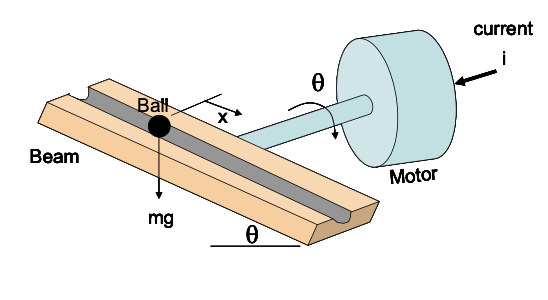
\includegraphics[width=0.4\textwidth]{images/intro_illustration.png}
    \caption{Illustration of the system}
    \label{fig:illustration}
\end{figure}

Following this, using the \textit{Root Locus method}, the necessary PD parameters are derived in accordance with the design requirements that make the system not only stable but also compliant with various constraint such as using an upper bound for settling time or percent overshoot.